\documentclass[tikz,border=5pt]{standalone}
\usepackage{amsmath}
\usetikzlibrary{arrows.meta}

\definecolor{inFill}{HTML}{DCE9F7}
\definecolor{inLine}{HTML}{2563EB}
\definecolor{grFill}{HTML}{DCFCE7}
\definecolor{grLine}{HTML}{15803D}
\definecolor{gyFill}{HTML}{F3F4F6}
\definecolor{gyLine}{HTML}{6B7280}
\definecolor{orFill}{HTML}{FFEDD5}
\definecolor{orLine}{HTML}{C2410C}
\definecolor{amFill}{HTML}{FEF3C7}
\definecolor{amLine}{HTML}{B45309}
\definecolor{lvFill}{HTML}{F3E8FF}
\definecolor{lvLine}{HTML}{7E22CE}
\definecolor{slate}{HTML}{374151}

\begin{document}
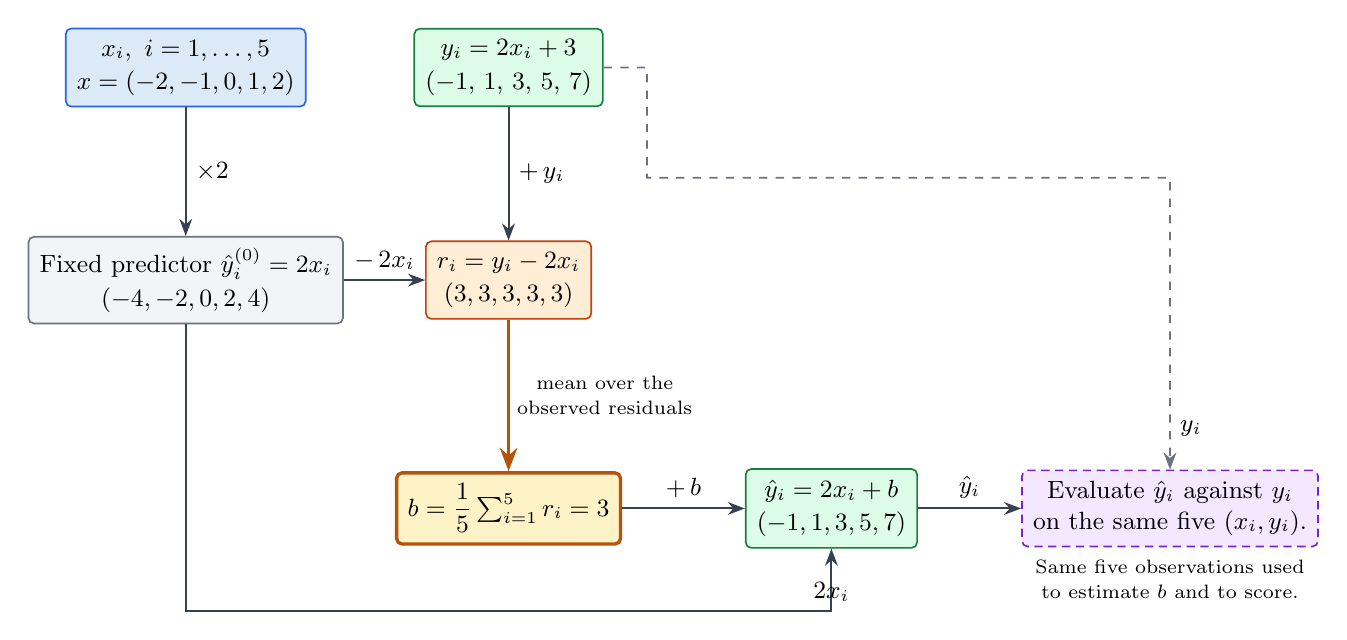
\begin{tikzpicture}[
  font=\small,
  box/.style={rounded corners=2pt, line width=0.6pt, align=center, inner sep=4pt},
  arr/.style={draw=slate, line width=0.7pt, -{Stealth}},
  note/.style={align=center, font=\fontsize{7.5}{9}\selectfont}
]

% ---------------- Nodes ----------------
\node[box, fill=inFill, draw=inLine] (input) at (0,7.0)
  {$x_i,\ i=1,\dots,5$\\[1pt] $x=(-2,-1,0,1,2)$};

\node[box, fill=grFill, draw=grLine] (target) at (4.1,7.0)
  {$y_i = 2x_i + 3$\\[1pt] $(-1,\,1,\,3,\,5,\,7)$};

\node[box, fill=gyFill, draw=gyLine] (baseline) at (0,4.3)
  {Fixed predictor $\hat{y}_i^{(0)} = 2x_i$\\[1pt] $(-4,-2,0,2,4)$};

\node[box, fill=orFill, draw=orLine] (residual) at (4.1,4.3)
  {$r_i = y_i - 2x_i$\\[1pt] $(3,3,3,3,3)$};

\node[box, fill=amFill, draw=amLine, line width=1.2pt] (mean) at (4.1,1.4)
  {$b = \dfrac{1}{5}\sum_{i=1}^{5} r_i = 3$};

\node[box, fill=grFill, draw=grLine] (corrected) at (8.2,1.4)
  {$\hat{y}_i = 2x_i + b$\\[1pt] $(-1,1,3,5,7)$};

\node[box, fill=lvFill, draw=lvLine, dash pattern=on 3pt off 2pt] (eval) at (12.5,1.4)
  {Evaluate $\hat{y}_i$ against $y_i$\\on the same five $(x_i, y_i)$.};

% ---------------- Edges ----------------
% Input -> Baseline
\draw[arr] (input.south) -- (baseline.north)
  node[midway, right] {$\times 2$};

% Target -> Residual (top anchor)
\draw[arr] (target.south) -- (residual.north)
  node[midway, right] {$+\,y_i$};

% Baseline -> Residual (left anchor)
\draw[arr] (baseline.east) -- (residual.west)
  node[midway, above] {$-\,2x_i$};

% Residual -> Mean residual (emphasized amber dependency)
\draw[draw=amLine, line width=1.2pt, -{Stealth}] (residual.south) -- (mean.north)
  node[midway, right, note, inner sep=2.5pt] {mean over the\\observed residuals};

% Mean -> Corrected (additive correction)
\draw[arr] (mean.east) -- (corrected.west)
  node[midway, above] {$+\,b$};

% Baseline feed: drop, run below Row 3, rise into corrected prediction
\draw[arr] (baseline.south) -- (0,0.1) -- (8.2,0.1) -- (corrected.south)
  node[pos=0.62, below] {$2x_i$};

% Corrected -> Evaluation
\draw[arr] (corrected.east) -- (eval.west)
  node[midway, above] {$\hat{y}_i$};

% Target -> Evaluation (dashed gray elbow along upper margin)
\draw[draw=gyLine, line width=0.7pt, dashed, -{Stealth}]
  (target.east) -- ++(0.55,0) -- ++(0,-1.4) -- (12.5,5.6) -- (eval.north)
  node[pos=0.86, right] {$y_i$};

% Reuse callout beneath the evaluation node
\node[note] at (12.5,0.5) {Same five observations used\\to estimate $b$ and to score.};

\end{tikzpicture}
\end{document}